\newpage
\onecolumn
\begin{comment}
\section{Proof of Lemma~\ref{lemma:red:hf}}
\label{sec:lem_red_obj}

We first notice that by the definition~\ref{eq:discretized} of $\ell_\alpha$, we have that
\begin{align*}
\E_D[\ell(Y,f(X))] - \ell(y,\tfrac{\alpha}{2}) &= |\calZ| \E_{D,Z} [w(Y,Z) h_f(X,Z)] = |\calZ| \E_{D,Z} [|w(Y,Z)|\sign(w(Y,Z)) h_f(X,Z)]\\
&= |\calZ| \E_{D,Z} [W'\ind(Y' \ne h_f(X')) - (1-Y')W'],
\end{align*}
%
where the last equality is clear when $Y' = \ind(w(Y,Z) > 0$ is 1, and can be easily checked in the case when it is 0. Finally, noting that the offset on the RHS is again independent of $h$ completes the proof.
\end{comment}

\section{Proof of Lemma~\ref{lemma:red:hf}}

We begin by rewriting the loss $\ell_\alpha$ as a cost-sensitive classification loss. First, we use the telescoping trick to obtain
%
\begin{align*}
\ell_{\alpha}(y,u)
&
 =\ell\BigParens{\undery,\floors{u}_\alpha\!+\tfrac{\alpha}{2}}
\\
&
=\ell(\undery,\tfrac{\alpha}{2})
    +\sum_{z\in\calZ}
     \BigBracks{
     \underbrace{\ell\BigParens{\undery,z+\tfrac{\alpha}{2}}-\ell\BigParens{\undery,z-\tfrac{\alpha}{2}}
     }_{c(\undery,z)/N}
     }
     \ind\braces{u\ge z}.
\end{align*}

Now plugging in $u=\underf(x)$ and using the fact that for $z\in\calZ$, we have $\ind\set{\underf(x)\ge z}=\ind\set{f(x)\ge z}=h_f(x,z)$, we obtain
%
\begin{align}
\label{eq:loss:hf}
  \ell_\alpha(y,\underf(x))
&
  =\ell(\undery,\tfrac{\alpha}{2})+\frac{1}{N}\sum_{z\in\calZ} c(\undery,z)h_f(x,z).
\end{align}
%
Thus, ignoring the constant $\ell(\undery,\tfrac{\alpha}{2})$, the loss $\ell_\alpha$ can be viewed as the cost-sensitive error of the classifier $h_f$.

For $z\in\calZ$, we can rewrite $\gamma_{a,z}(\underf)$ as
%
\begin{align}
\notag
\gamma_{a,z}(\underf)
  &= \P[\underf(X)\ge z\given A=a] - \P[\underf(X)\ge z]
\\
\label{eq:gamma:hf}
  &= \E[h_f(X,z)\given A=a] - \E[h_f(X,z)]
\\
\notag
  &=\gamma_{a,z}(h_f),
\end{align}
%
completing the proof of the lemma.

\section{Iteration Complexity of Algorithm~\ref{alg:regred:sp}}

\begin{theorem}
\label{thm:alg:sp}
\Alg{regred:sp} terminates in at most $\frac{16 B^2\log(2\card{\calA}\cardZ+1)}{\nu^2}$ iterations. Furthermore,
if $Q$ is any feasible point of \eqref{eq:prob:sp:empirical} then the solution $\hQ$ returned by \Alg{regred:sp} satisfies:
%
\begin{align*}
   \hcost(\hQ)
   &\le
   \hcost(Q)+2\nu
\\
   \bigAbs{\hgamma_{a,z}(\hQ)}
   &\le\heps_{a}+\frac{2+2\nu}{B}
\quad
\text{for all $a\in\calA$, $z\in\calZ$.}
\end{align*}
\end{theorem}

\begin{proof}
This result is essentially a corollary of Theorem 1, and Lemmas 2 and 3 of \citet{agarwal2018reductions}. Specifically, we note that the constraints appearing in our problem~\eqref{eq:prob:sp:empirical} can be cast in their general framework along the lines of their Example 1, with a total of $2\cardA\cardZ$ constraints.
%
%The only difference from Example 1 of their paper is that now we have $2\card{\Attr}$ constraints for each choice of $z \in \calZ$.
%
Following their Example 3, we obtain that the maximal constraint violation $\rho$, needed in their Theorem 1, is at most 2. We further observe that the violation of the i.i.d.\ structure by explicit averaging over $z$ values does not impact their optimization analysis in any way.
%
Therefore, their Theorem 1 with $\rho=2$ implies that our Algorithm~\ref{alg:regred:sp} finds a $\nu$-approximate saddle point of the Lagrangian in at most $\frac{16 B^2\log(2\card{\calA}\cardZ+1)}{\nu^2}$ iterations as desired.

To bound $\hcost(\hQ)$ and $\bigAbs{\hgamma_{a,z}(\hQ)}$ we appeal to their Lemmas 2 and 3. First note that
their approach applies to the objective of our problem~\eqref{eq:prob:sp:empirical} as long as the costs $c(y,z)$ are in $[0,1]$ (see their footnote 4). However, in our case, these can be in $[-1,1]$ (see Eq.~\ref{eqn:costs}). This does not affect their Theorem 1 and Lemma 2, but their Lemma 3 now holds with the right-hand side equal to $\frac{2+2\nu}{B}$ instead of $\frac{1+2\nu}{B}$. Their Lemma 2 immediately yields the bound $\hcost(\hQ)\le\hcost(Q)+2\nu$, whereas the modified Lemma 3 yields the bound
$\bigAbs{\hgamma_{a,z}(\hQ)}
 \le\heps_{a}+\frac{2+2\nu}{B}$ for all $a,z$, finishing the proof.
%
%
%
%While we use a weighted error, the weights (that is, the absolute values $\abs{c(y,z)}$) are bounded in $[0,1]$ (see Eq.~\ref{eqn:costs}) so that the boundedness properties of the lagrangian stay identical. We can now directly invoke Theorem 1 in their paper with $\rho = 2$ to bound the rate of convergence of Algorithm~\ref{alg:regred:sp} which gives the stated iteration complexity bound for attaining a $\nu$-approximate saddle point of the Lagrangian. Finally converting from a $\nu$-approximate saddle point to error and constraint violations follows from Lemma 2 and 3 of \citet{agarwal2018reductions} and only uses boundedness and non-negativity of the error, which still holds for our costs.
\end{proof}

\section{Proof of Theorem~\ref{thm:main:sp}}
\label{app:thm:main:sp}

Before proving the theorem, we recall a standard definition of the Rademacher complexity of a class of functions, which plays an important role in our deviation bounds. Let $\calG$ be a class of functions $g:\calU\to\R$ over some space $\calU$. Then the (worst-case) Rademacher complexity of $\calG$ is defined as:
\begin{equation}
R_n(\calG)
\coloneqq
\sup_{u_1,\ldots,u_n \in \calU} \E_{\sigma} \left[\sup_{g \in \calG} \left|\frac{1}{n} \sum_{i=1}^n \sigma_i g(u_i)\right|\right],
\label{eqn:rademacher}
\end{equation}
%
where the expectation is over the i.i.d.\ random variables $\sigma_1,\ldots,\sigma_n$ with $\P(\sigma_i = 1) = \P(\sigma_i = -1) = 1/2$.

The Rademacher complexity of a class $\calG$ can be used to obtain uniform bounds of any Lipschitz continuous
transformations of $g\in\calG$ as follows:
%
\begin{lemma}%[Concentration of moments]
\label{lemma:dev}
Let $D$ be a distribution over a pair of random
variables $(S,U)$ taking values in $\calS\times\calU$.
Let $\calG$ be a class of functions $g:\calU\to[0,1]$, and let $\phi:\calS\times[0,1]\to[-1,1]$ be a contraction in its second argument, i.e.,
for all $s\in\calS$ and all $t,t'\in[0,1]$, $\abs{\phi(s,t)-\phi(s,t')}\le\abs{t-t'}$.
Then with probability at least $1-\delta$, for all $g\in\calG$,
  \[
  \BigAbs{
     \Ehat\bigBracks{\phi(S,g(U))}-\E\bigBracks{\phi(S,g(U))}
  }
  \le
     4R_n(\calG) + \frac{2}{\sqrt{n}} + \sqrt{\frac{2\ln(2/\delta)}{n}}
\enspace,
  \]
where the expectation is with respect to $D$ and the empirical expectation is based on $n$ i.i.d.\ draws from $D$. If $\phi$ is also linear in its second argument then a tighter bound holds, with $4R_n(\calG)$ replaced by $2R_n(\calG)$.
%%
%% if phi is to [a,b] then the final term \sqrt{\frac{.}{n}} can be multiplied by (b-a)/2
%%
\end{lemma}
\begin{proof}
Let $\Phi\coloneqq\set{\phi_g}_{g\in\calG}$ be the class of functions $\phi_g: (s,u)\mapsto \phi(s,g(u))$.
By Theorem 3.2 of \citet{BoucheronBoLu05}, we then
have with probability at least $1-\delta$, for all $g$,
%
\begin{equation}
\label{eqn:phi:bound}
  \BigAbs{
     \Ehat\bigBracks{\phi(S,g(U))}-\E\bigBracks{\phi(S,g(U))}
  }
  =
  \BigAbs{\Ehat[\phi_g]-\E[\phi_g]}
  \le
  2 R_n(\Phi)
  +
  \sqrt{\frac{2\ln(2/\delta)}{n}}
\enspace.
\end{equation}
%
We will next bound $R_n(\Phi)$ in terms of $R_n(\calG)$. For a fixed tuple $(s_1,u_1),\dotsc,(s_n,u_n)$, we have
%
\begin{align*}
 \E_\sigma\Bracks{
     \sup_{g \in \calG}  \Abs{\sum_{i=1}^{n} \sigma_i \phi(s_i,g(u_i)) }
 }
&
\le
 \E_\sigma\Bracks{
     \sup_{g \in \calG}  \Abs{\sum_{i=1}^{n} \sigma_i \BigParens{\phi(s_i,g(u_i))-\phi(s_i,0)} }
 }
 +
 \sqrt{n}
\\
&
\le
 2\E_\sigma\Bracks{
     \sup_{g \in \calG}  \Abs{\sum_{i=1}^{n} \sigma_i g(u_i)}
 }
 +
 \sqrt{n}
\end{align*}
%
where the first inequality follows from Theorem 12(5) of~\citet{BartlettMe02} and the last inequality follows from the contraction principle of~\citet{LedouxTa91}, specifically their Theorem 4.12.
Dividing by $n$ and taking a supremum over $(s_1,u_1),\dotsc,(s_n,u_n)$ yields the bound
\[
  R_n(\Phi)\le 2R_n(\calG)+\frac{1}{\sqrt{n}}.
\]
Together with the bound~\eqref{eqn:phi:bound}, this proves the lemma for an arbitrary contraction $\phi$. If $\phi$ is linear in its second argument, we get a tighter bound by invoking Theorem 4.4 of~\citet{LedouxTa91} instead of their Theorem 4.12.
\end{proof}

Our proof largely follows the proof of Theorems~2 and~3 of \citet{agarwal2018reductions}. We first use \Lemma{dev} to show that by solving the empirical problem~\eqref{eq:prob:sp:empirical}, we also obtain an approximate solution of the corresponding population problem:
%
\begin{align}
\label{eq:prob:sp}
  \min_{\mathclap{Q\in\Delta(\calH)}}\;\cost(Q)
\text{ s.t. }
  \bigAbs{\gamma_{a,z}(Q)}\le\eps_a
\;\;
  \text{$\forall a\in\calA, z\in\calZ$.}
%
% \min_{Q\in\Delta(\calH)} \cost(Q)
%\text{ s.t. }
%  \bigAbs{\gamma_{a,z}(Q)}\le\eps_a
%  \text{ $\forall$ $a\in\calA$, $z\in\calZ$.}
\end{align}
%
The theorem will then follow by invoking the equivalence between problem~\eqref{eq:prob:sp} and the discretized
fair regression~\eqref{eq:fair-reg:sp:apx}, and adding up various approximation errors.

\paragraph{Bounding empirical deviations in the cost and constraints.}
To bound the deviations in the cost, we need to be a bit careful, because the definition of $\hcost$ mixes
the empirical expectation over the data with the averaging over $z\in\calZ$. For the analysis, we therefore
define
\[
   \hcost_z(h)=\Ehat\bigBracks{c(\underY,z)h(X,z)}
\quad
\text{and}
\quad
   \cost_z(h)=\E\bigBracks{c(\underY,z)h(X,z)}.
\]
Since $c(\underY,z)\in[-1,1]$, we can invoke \Lemma{dev} with $S=c(\underY,z)$, $U=(X,z)$, $\calG=\calH$, and $\phi(s,t)=st$ to obtain that with probability at least $1-\delta/2$ for all $z\in\calZ$ and all $h\in\calH$
\[
  \BigAbs{\hcost_z(h)-\cost_z(h)}
  \le
  2R_n(\calH)+\frac{2}{\sqrt{n}}+\sqrt{\frac{2\ln(4N/\delta)}{n}}
  =
  \otil(n^{-\beta})
,
\]
where the last equality follows by Assumption~\ref{ass:samples} and the setting $\cardZ\propto n^\beta$.
Taking an average over $z\in\calZ$ and a convex combination according to any $Q\in\Delta(\calH)$, we obtain by Jensen's inequality
that with probability at least $1-\delta/2$ for all $Q\in\Delta(\calH)$
%
\begin{equation}
\label{eq:dev:cost}
  \bigAbs{\hcost(Q)-\cost(Q)}
  =
  \otil(n^{-\beta})
.
\end{equation}

To bound the deviations in the constraints, we invoke \Lemma{dev} with $S=1$, $U=(X,z)$, $\calG=\calH$, and $\phi(s,t)=st$, but apply it to the data distribution conditioned on $A=a$. We thus obtain that with with probability at least $1-\delta/2$ for all $a\in\calA$, $z\in\calZ$, and $h\in\calH$
\[
  \BigAbs{\hgamma_{a,z}(h)-\gamma_{a,z}(h)}
  \le
  2R_{n_a}(\calH)+\frac{2}{\sqrt{n_a}}+\sqrt{\frac{2\ln(4\cardA N/\delta)}{n_a}}
%  =
%  \otil(n_a^{-\beta})
.
\]
By Jensen's inequality this also means
that with probability at least $1-\delta/2$ for all $a\in\calA$, $z\in\calZ$, and $Q\in\Delta(\calH)$
%
\begin{equation}
\label{eq:dev:gamma}
  \bigAbs{\hgamma_{a,z}(Q)-\gamma_{a,z}(Q)}
  \le
  2R_{n_a}(\calH)+\frac{2}{\sqrt{n_a}}+\sqrt{\frac{2\ln(4\cardA N/\delta)}{n_a}}
%  =
%  \otil(n_a^{-\beta})
.
\end{equation}
%
In the remainder of the analysis, we assume that \Eqs{dev:cost}{dev:gamma} both hold, which occurs with probability at least $1-\delta$ by the union bound.

\paragraph{Putting it all together.}

Given the settings of $\nu$, $B$ and $N$, we obtain by \Thm{alg:sp} that Algorithm~\ref{alg:regred:sp} terminates in $\order\bigParens{n^{4\beta}\ln (n^\beta\card{\calA})}$ iterations, as desired, and returns a distribution $\hQ$ which compares favorably
with any feasible point $Q$ of the empirical problem~\eqref{eq:prob:sp:empirical}, meaning that for
any such $Q$, we have
%
\begin{align}
\label{eq:sp:app:1}
   \hcost(\hQ)
   &\le
   \hcost(Q)+\order(n^{-\beta})
\\
\label{eq:sp:app:2}
   \bigAbs{\hgamma_{a,z}(\hQ)}
   &\le\heps_{a}+\order(n^{-\beta})
\quad
\text{for all $a\in\calA$, $z\in\calZ$.}
\end{align}
%
Now bounding $\hcost(\hQ)$ and $\hcost(Q)$ in \Eq{sp:app:1} via the uniform convergence bound~\eqref{eq:dev:cost}, we obtain
%
\begin{align}
\label{eq:sp:app:3}
   \cost(\hQ)
&
   \le
   \cost(Q)+\otil(n^{-\beta}).
\intertext{%
Similarly, bounding $\hgamma_{a,z}(\hQ)$ via the bound~\eqref{eq:dev:gamma} and
$\heps_a\le\eps_a+\otil(n_a^{-\beta})$ via Assumption~\ref{ass:samples} and our setting of $C'$, we obtain
}
\label{eq:sp:app:4}
   \bigAbs{\gamma_{a,z}(\hQ)}
&
   \le\eps_{a}+\otil(n_a^{-\beta})
\quad
\text{for all $a\in\calA$, $z\in\calZ$.}
\end{align}

Above, we assumed that $Q$ was a feasible point of the empirical problem~\eqref{eq:prob:sp:empirical}. However, assuming that \Eq{dev:gamma} holds, any
feasible solution of the population problem~\eqref{eq:prob:sp} is also feasible in
the empirical problem~\eqref{eq:prob:sp:empirical} thanks to our setting of $C'$. Thus,
\Eqs{sp:app:3}{sp:app:4} show that the solution $\hQ$ is approximately feasible and approximately optimal in the population problem~\eqref{eq:prob:sp}. It remains to relate $\hQ$ to the original fair regression problem~\eqref{eq:fair-reg:sp}.

First, by \Lemma{red:hf} and \Eqs{sp:app:3}{sp:app:4}, we can interpret $\hQ$ as a distribution over the set of discretized regressors $\underF$ and obtain that for all $\underQ\in\Delta(\underF)$ that
are feasible in the discretized fair regression problem~\eqref{eq:fair-reg:sp:apx}, we have
%
\begin{align}
\label{eq:sp:app:5}
   \loss_\alpha(\hQ)
&
   \le
   \loss_\alpha(\underQ)+\otil(n^{-\beta})
\\
\label{eq:sp:app:6}
   \bigAbs{\gamma_{a,z}(\hQ)}
&
   \le\eps_{a}+\otil(n_a^{-\beta})
\quad
\text{for all $a\in\calA$, $z\in[0,1]$,}
\end{align}
%
where in \Eq{sp:app:6} we have expanded the domain $z\in\calZ$ to $z\in[0,1]$ thanks to \Eq{gamma:apx}. Finally, by substituting the solution $\underQ^*$ of problem~\eqref{eq:fair-reg:sp:apx} as $\underQ$ in \Eq{sp:app:5} and
applying \Thm{sp:apx}, we obtain that for any $Q^*\in\Delta(\calF)$ that is feasible in the discretized fair regression problem~\eqref{eq:fair-reg:sp:apx}, we have
%
\begin{equation}
\label{eq:sp:app:7}
   \loss(\hQ)
   \le
   \loss(Q^*)+\alpha+\otil(n^{-\beta})=\loss(Q^*)+\otil(n^{-\beta}),
\end{equation}
%
where the last equality follows by our setting $\alpha=1/N=O(n^{-\beta})$. The theorem now follows from \Eqs{sp:app:7}{sp:app:6}.

%Let $Q^*\in\Delta(\calF)$ be any feasible point of the original fair regression problem~\eqref{eq:fair-reg:sp} and let $\underQ^*$ be the matching distribution over $\underF$.

\section{Algorithm for Fair Regression under Bounded Group Loss}
\label{sec:app:alg:ep}

In this section we provide a detailed pseudocode of our algorithm for fair regression under \epshort, described at a high level in Section~\ref{sec:max-loss-bound}.

\begin{algorithm}[t]
\caption{Fair regression with \ep}
\label{alg:regred:ep}
  \begin{algorithmic}[1]
    \Statex{Input:~~training examples $\braces{(X_i,Y_i,A_i)}_{i=1}^n$, slacks in fairness constraint $\hzeta_{a}\in[0,1]$, bound $B$, convergence threshold $\nu$}
%%%% \eps = \eps^*+c/\sqrt{n}
%%%% M \propto 1/\eps
%%%% T \propto 1/\eps^2
%%%% \eta \propto M/\sqrt{T} = const
\smallskip
    \Statex{Define best-response functions:}
    \Statex{~\hphantom{Input:}~$\BestF(\vlambda)\coloneqq\argmin_{f\in\calF} \LE(f,\vlambda)$}
    \Statex{~\hphantom{Input:}~$\BestLambda(Q)\coloneqq\argmax_{\vlambda\ge 0,\,\norm{\vlambda}_1\le B} \LE(Q,\vlambda)$}
\smallskip
    \State{Set learning rate $\eta=\nu/(2B)$}
    \State{Set $\vtheta_1=\vzero\in\R^{\card{\calA}}$}
\smallskip
    \For{$t=1, 2, \ldots$}
%\Statex{\hspace{\algorithmicindent}%
 %               \textit{// Compute $\vlambda_t$ from $\vtheta_t$ and find the best response $h_t$}}
%\textit{// Obtain the exponentiated-gradient iterate $\vlambda_t$,}}
%\Statex{\hspace{\algorithmicindent}%
%        \hphantom{\textit{// }}%
%        \textit{play it, and obtain the best response $f_t$}}
\smallskip
    \ForAll{$a$} \hfill \textit{// Compute $\vlambda_t$ from $\vtheta_t$ and find the best response $f_t$}
%    \State{\textbf{for all} $a,z$ \textbf{do}}
    \State{$\lambda_{t,a}\gets B\,\exp\braces{\theta_{t,a}}/\left(1+\sum_{a}\exp\braces{\theta_{t,a}}\right)$}
    \EndFor
    \State{$f_t\gets\BestF(\vlambda_t)$}
\medskip
%\Statex{\hspace{\algorithmicindent}%
%        \textit{// Calculate the current approximate saddle point}}
%\Statex{\hspace{\algorithmicindent}%
%        \hphantom{\textit{// }}%
%        \textit{(the average joint play)}}
%\medskip
    \State{$\hQ_t\gets\frac{1}{t}\sum_{t'=1}^t f_{t'},
      \quad
            \hvlambda_t\gets\frac{1}{t}\sum_{t'=1}^t \vlambda_{t'}$ \hfill \textit{// Calculate the current approximate saddle point}}
%\medskip
%\Statex{\hspace{\algorithmicindent}%
%        \textit{// Check the suboptimality of $(\hQ_t,\hvlambda_t)$}}
%\Statex{\hspace{\algorithmicindent}%
%        \hphantom{\textit{// }}%
%        \textit{and terminate if below $\nu$}}
\medskip
    \State{$\overline{\nu}\gets \LE\bigParens{\hQ_t,\BestLambda(\hQ_t)}\;-\;\LE(\hQ_t,\hvlambda_t)$
           \hfill \textit{// Check the suboptimality of $(\hQ_t,\hvlambda_t)$}}
    \State{$\underline{\nu}\gets \LE(\hQ_t,\hvlambda_t)\;-\;\LE\bigParens{\BestF(\hvlambda_t),\hvlambda_t}$}
\medskip
    \If{$\max\set{\overline{\nu},\underline{\nu}}\le\nu$}
           \hfill \textit{// Terminate if converged}
    \smallskip
        \If{$\hgammaE(\hQ_t) \leq \hzeta_a + \tfrac{1+2\nu}{B}$ for all $a \in \calA$}
        \State{\textbf{return} $\hQ_t$}
        \Else
        \State{\textbf{return $\nullval$}}
        \EndIf
    \EndIf
%\medskip
%\Statex{\hspace{\algorithmicindent}%
%        \textit{// Apply the exponentiated-gradient update}}
\medskip
    \State{Set $\vtheta_{t+1}=\vtheta_t+\eta\hvgammaE(f_t)-\eta\hvzeta$\hfill \textit{// Apply the exponentiated-gradient update}}
    %\alekh{Should this be a $+ \eta\hveps$?} MD: no
    \EndFor
\end{algorithmic}
\end{algorithm}


\section{Proof of Theorem~\ref{thm:main:ep}}

The analysis of Algorithm~\ref{alg:regred:ep} proceeds similarly to the analysis of Algorithm~\ref{alg:regred:sp}.

\paragraph{Iteration complexity.} Similarly to our analysis of Algorithm~\ref{alg:regred:sp} in \Thm{alg:sp},
we can appeal to Theorem 1, and Lemmas 2 and 3 of \citet{agarwal2018reductions}. While our objective and constraints are for the distributions $Q$ over $[0,1]$-valued predictors $f\in\calF$, whereas their analysis is for distributions over $\set{0,1}$-valued classifiers, we can still directly use their Theorem 1, and Lemmas 2 and 3, because they only rely on the bilinear structure of the Lagrangian with respect to $Q$ and $\vlambda$ and the boundedness of the objective and constraints, which all hold in our setting. The maximal constraint violation, needed in their Theorem 1, is $\rho\le 1$. Therefore, their Theorem 1 implies that Algorithm~\ref{alg:regred:ep} terminates in at most $4B^2\ln(\cardA + 1)/\nu^2=O(n^{4\omega}\ln\cardA)$ iterations and
finds a $\nu$-approximate saddle point $\hQ$ of problem~\eqref{eq:minmax:ep}, albeit sometimes it ends up returning $\nullval$ instead of $\hQ$. To prove the theorem we consider two cases.

\paragraph{Case I: There is a feasible solution $Q^*$ to the original problem~\eqref{eq:fair-reg:ep}.}
Given the settings of $\nu$ and $B$, and using Lemmas 2 and 3 of \citet{agarwal2018reductions}, we obtain that the $\nu$-approximate saddle point $\hQ$ of the empirical problem~\eqref{eq:minmax:ep} satisfies
%
\begin{align}
\label{eq:ep:app:1}
  \hloss(\hQ)
  &\le
  \hloss(Q) + 2\nu
%  =
%  \hloss(Q) + O(n^{-\omega})
\\
\label{eq:ep:app:2}
  \hgammaE_a(\hQ)
  &
  \le
  \hzeta_a + \frac{1+2\nu}{B}
%  =
%  \hzeta_a + O(n^{-\omega})
  \quad
  \text{for all $a\in\calA$,}
\end{align}
%
for any distribution $Q$ feasible in the empirical problem~\eqref{eq:fair-reg:ep:emp}. \Eq{ep:app:2} implies that in this case the algorithm returns $\hQ\ne\nullval$. It remains to argue that statements similar
to~\eqref{eq:ep:app:1} and~\eqref{eq:ep:app:2} hold for true expectations rather than just empirical expectations.

To turn the statements~\eqref{eq:ep:app:1} and~\eqref{eq:ep:app:2} into matching population versions, we use the concentration result of \Lemma{dev} similarly as in the proof of \Thm{main:sp}. Specifically, we invoke \Lemma{dev} with $S=Y$, $U=X$, $\calG=\calF$, and $\phi(s,t)=\ell(s,t)$, separately for the data distribution (with failure probability $\delta/2$) and the data distribution
conditioned on each $A=a$ (with failure probabilities $\delta/(2\cardA)\,$). We thus obtain that with probability at least $1-\delta$, for all $Q\in\Delta(\calF)$,
%
\begin{align*}
  \bigAbs{\hloss(Q)-\loss(Q)}
  &\le
  4R_{n}(\calF)+\frac{2}{\sqrt{n}}+\sqrt{\frac{2\ln\parens{4/\delta}}{n}}
\\
  \bigAbs{\hgammaE_a(Q)-\gammaE_a(Q)}
  &\le
  4R_{n_a}(\calF)+\frac{2}{\sqrt{n_a}}+\sqrt{\frac{2\ln\parens{4\cardA/\delta}}{n_a}}
  \quad
  \text{for all $a\in\calA$.}
\end{align*}
%
By Assumption~\ref{ass:samples:ep} and our setting of $C'$, this implies that with probability at least $1-\delta$, for all $Q\in\Delta(\calF)$,
%
\begin{align}
\label{eq:ep:app:3}
  \bigAbs{\hloss(Q)-\loss(Q)}
  &=\otil(n^{-\omega})
\\
\label{eq:ep:app:4}
  \bigAbs{\hgammaE_a(Q)-\gammaE_a(Q)}
  &\le C' n_a^{-\omega}
  \quad
  \text{for all $a\in\calA$.}
\end{align}
%
We continue the analysis assuming that the uniform convergence bounds~\eqref{eq:ep:app:3} and~\eqref{eq:ep:app:4} both hold. Instantiating the bound~\eqref{eq:ep:app:3} for $\hloss(Q)$ and $\hloss(\hQ)$ in \Eq{ep:app:1} yields,
for any $Q$ feasible in the empirical problem~\eqref{eq:fair-reg:ep:emp},
%
\begin{align}
\label{eq:ep:app:5}
  \loss(\hQ)
  &\le
  \loss(Q) + 2\nu + \otil(n^{-\omega})
  =
  \loss(Q) + \otil(n^{-\omega}),
\intertext{%
where the last equality follows by our setting of $\nu$. Similarly, instatianting the bound~\eqref{eq:ep:app:4} for $\hgammaE_a(\hQ)$ in \Eq{ep:app:2} yields}
\label{eq:ep:app:6}
  \gammaE_a(\hQ)
  &
  \le
  \hzeta_a + \frac{1+2\nu}{B} + \otil(n_a^{-\omega})
  \le
  \zeta_a + \otil(n_a^{-\omega})
  \quad
  \text{for all $a\in\calA$,}
\end{align}
%
where the last inequality follows by our setting of $B$, $\nu$, and $C'$ as well as the bound
$\hzeta_a\le\zeta_a+C'n_a^{-\omega}$ from Assumption~\ref{ass:samples:ep}.

Above, we assumed that $Q$ was a feasible point of the empirical problem~\eqref{eq:fair-reg:ep:emp}. However, assuming that \Eq{ep:app:4} holds, any
feasible solution of the population problem~\eqref{eq:fair-reg:ep} is also feasible in
the empirical problem~\eqref{eq:fair-reg:ep:emp} thanks to our setting of $C'$. Thus,
\Eqs{ep:app:5}{ep:app:6} hold for any $Q^*$ feasible in~\eqref{eq:fair-reg:ep}, proving the theorem in this case.

\paragraph{Case II: There is no feasible solution $Q^*$ to the original problem~\eqref{eq:fair-reg:ep}.} In this case, the $\nu$-approximate saddle point $\hQ$ that the algorithm finds may still satisfy
%
\begin{equation}
\label{eq:ep:app:7}
  \hgammaE_a(\hQ)\le\hzeta_a + \frac{1+2\nu}{B}
  \quad
  \text{for all $a\in\calA$,}
\end{equation}
%
in which case the algorithm returns $\hQ$ and the theorem holds vacuously since here is no feasible point $Q^*$. If the found approximate saddle point does not satisfy \Eq{ep:app:7}, then the algorithm returns $\nullval$ and the theorem also holds.

\section{Details for Efficient Implementation of Algorithm~\ref{alg:regred:sp}}
\label{sec:app:impl}

On the high level, \Alg{regred:sp} keeps track of auxiliary vectors $\vtheta_t^+,\vtheta_t^-\in\R^{\cardA\cardZ}$. These are used to obtain the vector $\vlambda_t\in\R{2\cardA\cardZ}$ played by the $\vlambda$-player. The $Q$-player responds to $\vlambda_t$ by playing $h_t\in\calH$ (\Step{best:response}), which is used to update $\vtheta_t^\pm$. The average of $\vlambda_t$'s and $h_t$'s played so far is the candidate solution for the saddle-point problem
%
\begin{equation}
\label{eq:minmax}
\adjustlimits\min_{\;\;Q\in\Delta\;\;}\max_{\vlambda\ge\vzero,\,\norm{\vlambda}_1\le B} L(Q,\vlambda).
\end{equation}
%
The algorithm checks the suboptimality of this solution and terminates once the convergence $\nu$ is reached (\StepsRange{conv:check}).

%updating $\vtheta_t^\pm$ (Steps 2, 13, 14), which are transformed, at the beginning of each iteration, into the vector $\vlambda_t$ (Steps 4--7), which is played by the $\vlambda$-player. The $Q$-player responds to $\vlambda_t$ by playing $h_t\in\calH$ (Step 8).

The updates of
$\vtheta_t^+$ and $\vtheta_t^-$ (\Step{theta:update}) run in time $O(\cardA\cardZ)$ assuming that $\vgamma(h_t)$ has already been calculated. Similarly, the transformation of $\vtheta_t^+$ and $\vtheta_t^-$ to $\vlambda_t$ (\StepsRange{lambda:update}) runs in time $O(\cardA\cardZ)$, because the denominator is the same across all coordinates and so it needs to be computed only once. We next show that the remaining operations, except for the two $\BestH$ calls, run in time $\order(n\log n+\card{\calA}\cardZ)$.

%The bulk of the running time is in calculating the best response $h_t$ and in checking the suboptimality of the computation includes the $\BestH$ call in Step 8, and the Lagrangian calculations in Steps 10--11.

%We begin by bounding the runtime of evaluation of $\hcost(h_f)$ and $\hvgamma(h_f)$ for any $h_f\in\calH$, then continue by bounding the runtime of
%evaluation of $L(h_f,\vlambda)$ and $L(\hQ_t,\vlambda)$ for any $h_f$ and $\vlambda$, and finish by analyzing the runtime of $\BestLambda$ and $\BestH$. All of
%the remaining operations run in time $\order(\card{\calA}\card{\calJ}\cardZ)$.

\textbf{Computation of $\hcost(h_f)$ and $\hvgamma(h_f)$.} This computation is implicit in the calculation of Lagrangian in Steps~\ref{step:L:bestL}--\ref{step:L:bestH}, and also in the updates of $\vtheta_t^+$ and $\vtheta_t^-$ in \Step{theta:update}. By \Eq{loss:hf},
\[
  \hcost(h_f)=\Ehat\BigBracks{\ell_\alpha(Y,\underf(X))-\ell\bigParens{Y,\,\tfrac{\alpha}{2}}},
\]
so it can be calculated in time $\order(n)$ in a single pass over examples. To calculate $\hvgamma(h_f)$, we keep the training examples partitioned
into $\card{\calA}$ disjoint sets according to their protected attribute $A$. Let $n_{a}$ be the number of examples with $A=a$.
We sort these examples according to $f(X)$ in time $\order(n_{a}\log n_{a})$. Now going through these examples from the largest $f(X)$ value to the smallest allows us to calculate the conditional expectations
\[
  \Ehat[h_f(X,z)\given A=a] = \Phat[f(X)\ge z\given A=a]
\]
across all $z$ in time $\order(n_{a}+\cardZ)$. Since we need to do this for all $a\in\calA$,
the overall runtime is $\order(n\log n+\card{\calA}\cardZ)$. Finally, to
calculate $\hvgamma$ we also need expectations $\Ehat[h_f(X,z)]$, which can be obtained by taking weighted sums
of $\Ehat[h_f(X,z)\given A=a]$ in time $\order(\card{\calA}\cardZ)$. Altogether, the running time
of computing $\hcost(h_f)$ and $\hvgamma(h_f)$ is therefore $\order(n\log n+\card{\calA}\cardZ)$.

\textbf{Computation of $L(h_f,\vlambda)$ and $L(\hQ_t,\vlambda)$.} Lagrangian is evaluated in Steps~\ref{step:L:bestL}--\ref{step:L:bestH} to determine whether the algorithm has converged. Note that $L(Q,\vlambda)$ depends on $Q$ only through $\hcost(Q)$ and $\hvgamma(Q)$.
If we have already computed these, $L(Q,\vlambda)$ can be evaluated in time $\order(\card{\calA}\cardZ)$. To calculate $L(h_f,\vlambda)$ for an arbitrary
$h_f$, we first need to calculate $\hcost(h_f)$ and $\hvgamma(h_f)$, so the overall running time is $\order(n\log n+\card{\calA}\cardZ)$. To calculate
$L(\hQ_t,\vlambda)$, note that $\hcost(\hQ_t)=\frac{1}{t}\sum_{t'=1}^t\hcost(h_{t'})$, so we can obtain $\hcost(\hQ_t)$ from $\hcost(\hQ_{t-1})$ at the cost of evaluation
of $\hcost(h_t)$ and similarly for $\hvgamma(\hQ_t)$. Therefore, the first evaluation of the form $L(\hQ_t,\vlambda)$ takes time $\order(n\log n+\card{\calA}\cardZ)$
and each consequent evaluation takes time $\order(\card{\calA}\cardZ)$.

\textbf{Computation of $\BestLambda(\hQ_t)$.} The best response of the $\vlambda$-player is used in \Step{L:bestL} to determine the suboptimality of the current solution. Given an arbitrary $Q$, $\BestLambda(Q)$ returns
$\vlambda$ maximizing $L(Q,\vlambda)$ over $\vlambda\ge\vzero,\norm{\vlambda}_1\le B$. By first-order optimality, the optimizing $\vlambda$ is either $\vzero$ or puts all of its mass on the most
violated constraint among $\hgamma_{a,z}(Q)\le\heps_{a}$, $\hgamma_{a,z}(Q)\ge-\heps_{a}$. In particular,
let $\ve_{a,z}^+$ and $\ve_{a,z}^-$ denote the basis vectors corresponding to coordinates $\lambda_{a,z}^+$ and $\lambda_{a,z}^-$. The call to $\BestLambda(Q)$ first calculates
\[
  (a^*\!,z^*)=\smash{\argmax_{(a,z)}\bigBracks{\abs{\hgamma_{a,z}(Q)}-\heps_{a}}}
\]
and then returns
\[
   \begin{cases}
   B\ve_{a^*,z^*}^+
      &\text{if $\hgamma_{a^*\!,z^*}(Q)>\heps_{a^*}$}
   \\
   B\ve_{a^*,z^*}^-
      &\text{if $\hgamma_{a^*\!,z^*}(Q)<-\heps_{a^*}$}
   \\
   \vzero
      &\text{otherwise.}
   \end{cases}
\]
Thus, $\BestLambda(\hQ_t)$ can be calculated in time $\order(\card{\calA}\cardZ)$ as long as we have $\hvgamma(\hQ_t)$, whose computation we have already accounted for within the computation of the Lagrangian of the form $L(\hQ_t,\vlambda)$.

\subsection{Details for Reduction to Cost-sensitive Classification}

By definition of $\hgamma_{a,z}(h)$, we have
\begin{align}
\notag
\sum_{a,z}\lambda_{a,z}\hgamma_{a,z}(h)
&=
  \sum_{a,z}\lambda_{a,z}\Parens{\frac{1}{p_{a}}\Ehat\bigBracks{h(X,z)\ind\set{A=a}}
  - \Ehat\bigBracks{h(X,z)}}
\\
\notag
&=
  \Ehat\BiggBracks{
  N\E_Z\BiggBracks{
     \sum_{a}\lambda_{a,Z}\,h(X,Z)\Parens{\frac{\ind\set{A=a}}{p_{a}} - 1}
  }}
\\
\label{eq:hgamma:1}
&=
  \Ehat\biggBracks{
  N\E_Z\biggBracks{
     \biggParens{
     \frac{\lambda_{A,Z}}{p_A} -\!\sum_a\lambda_{a,Z}
     }
     h(X,Z)
  }}.
\end{align}
%
In particular, \Eqs{hcost}{hgamma:1} imply that the minimization of $L(h,\vlambda)$ is indeed equivalent to minimizing the right-hand side of \Eq{c:lambda} as claimed.

\subsection{Details for Reduction to Least-squares Regression}
\label{sec:app:impl:ls}

The construction of the least-squares regression data set begins with \Eq{c:lambda}, which states
that for $h_f\in\calH$
%
\begin{align}
%\notag
%&
  \hcost(h_f)
  +
  \sum_{a,z}\lambda_{a,z}\hgamma_{a,z}(h_f)
%\\
\label{eq:c:lambda:2}
%&\quad{}=
&\,=\,
  \frac1n\sum_{i\le n}\sum_{z\in\calZ}
     \frac1N c_{\vlambda}(\underY_i,A_i,z)h_f(X_i,z).
\end{align}
%
We will now rewrite the inner summation over $z$ as a loss function for the predictor $f$, parameterized by $\vlambda$. More precisely, for any $a\in\calA$ and $\ty\in\tcalY$, let the ``loss'' function for a prediction $u$ be defined as
\[
  g_{\vlambda}(\ty,a,u)=\sum_{z\in\calZ, z\le u}\frac1N c_{\vlambda}(\ty,a,z).
\]
Now consider a specific $i$ in \Eq{c:lambda:2}. Let $X\coloneqq X_i$, $A\coloneqq A_i$ and $\tY\coloneqq \underY_i$. Then the summation over $z$ for this specific $i$ can be written as
%
\begin{align*}
\sum_{z\in\calZ}
     \frac1N
     c_{\vlambda}(\tY,A,z)h_f(X,z)
&\,=\,
\sum_{z\in\calZ}
     \BigBracks{g_{\vlambda}(\tY,A,z)-g_{\vlambda}(\tY,A,z-\alpha)}\ind\set{f(X)\ge z}
\\
&\,=\,
  g_{\vlambda}(\tY,A,\floors{f(X)}_\alpha)
\\
&\,=\,
  g_{\vlambda}(\tY,A,f(X))
.
\end{align*}
%
%\aacomment{Ignoring the first term independent of $f$ in the telescoping?}
Plugging this back into \Eq{c:lambda:2}, we see that the minimization of \Eq{c:lambda:2} over $h\in\calH$ is equivalent to the minimization of the empirical loss under $g_{\vlambda}$ among $f\in\calF$:
\[
  \min_{f\in\calF}
  \Bracks{
  \frac1n\sum_{i=1}^n
     g_{\vlambda}(\underY_i,A_i,f(X_i))
  }.
\]
Solving this problem directly seems to require access to a generic optimization oracle. We instead use a heuristic, where we first pick
\[
  U_i\in\argmin_{u\in[0,1]} g_{\vlambda}(\underY_i,A_i,u)
\]
and then seek to solve the least-squares regression problem
\[
  \min\sum_{i\le n} (U_i-f(X_i))^2
.
\]
To obtain the values $U_i$ we first calculate the values $c_{\vlambda}(\ty,a,z)$ across all $\ty$, $a$, and $z$
in the overall time $\order(\card{\calA}\card{\tcalY} N)$. Then, using the definition of $g_{\vlambda}$, the minimizer
of $g_{\vlambda}(\ty,a,u)$ over $u$ can be found in time $\order(N)$ for each specific value of $\ty$ and $a$, so
all the minimizers can be precalculated in time $\order(\card{\calA}\card{\tcalY} N)$. Thus, preparing the data set for
the least-squares reduction takes time $\order(\card{\calA}\card{\tcalY} N)$ and the resulting regression data set
is of size $n$.\looseness=-1

\subsection{Details for Reduction to Risk Minimization under $\ell$}
\label{app:reduction:ell}

The same reasoning that yielded the reduction to the least-squares regression can be used to derive
a reduction to risk minimization under any loss $\ell(y,u)$ that is convex in $u$. We again begin with computing the minimizers $U_i$ for each $g_{\vlambda}(\underY_i, A_i, f(X_i))$ term. Now suppose that there are two values $\tY_{i,1},\tY_{i,2} \in [0,1]$ such that $\frac{\partial}{\partial u} \ell(\tY_{i,1},U_i) \leq 0$ and $\frac{\partial}{\partial u} \ell(\tY_{i,2},U_i) \geq 0$ (if $\ell$ is non-smooth, we can pick arbitrary elements of the subdifferential set). If no such pair exists, then it is not possible to obtain $f(X_i) = U_i$ by minimizing $\ell$ over any distribution of examples since the gradient can never vanish at $U_i$. However, if such a pair exists, we can induce weights $W_{i,1}, W_{i,2}\in[0,1]$ such that $W_{i,1} + W_{i,2} = 1$ and
\[\textstyle
  W_{i,1}\,\frac{\partial}{\partial u} \ell(\tY_{i,1},U_i) + W_{i,2}\,\frac{\partial}{\partial u} \ell(\tY_{i,2},U_i) = 0.
\]
Hence, we create two weighted examples for each $(X_i,A_i,Y_i)$ triple in our dataset, and solve
\[
\min_{f \in \calF}\,\sum_{i=1}^n\BigBracks{W_{i,1}\,\ell(\tY_{i,1}, f(X_i)) + W_{i,2}\,\ell(\tY_{i,2},f(X_i))}.
\]
%
For instance, for logistic loss, we can always pick $\tY_{i,1} = 0$, $\tY_{i,2} = 1$ and $W_{i,2} = U_i$. The complexity of this reduction is identical to that of the least-squares reduction above, but the resulting risk minimization problem might be better aligned with the original problem as the experiments
in Section~\ref{sec:experiments} show.


\section{Additional Experimental Results}
\label{app:exp}

In this section, we include further details on our experimental
evaluation.

\paragraph{Evaluation on the training sets.} In Figure~\ref{train} we
include the training performances of our algorithm and the baseline
methods, including the SEO method and the unconstrained
regressors. Our method generally dominated or closely matched the baseline
methods. The SEO method provided solutions that were not Pareto
optimal on the law school data set.

\begin{figure*}
  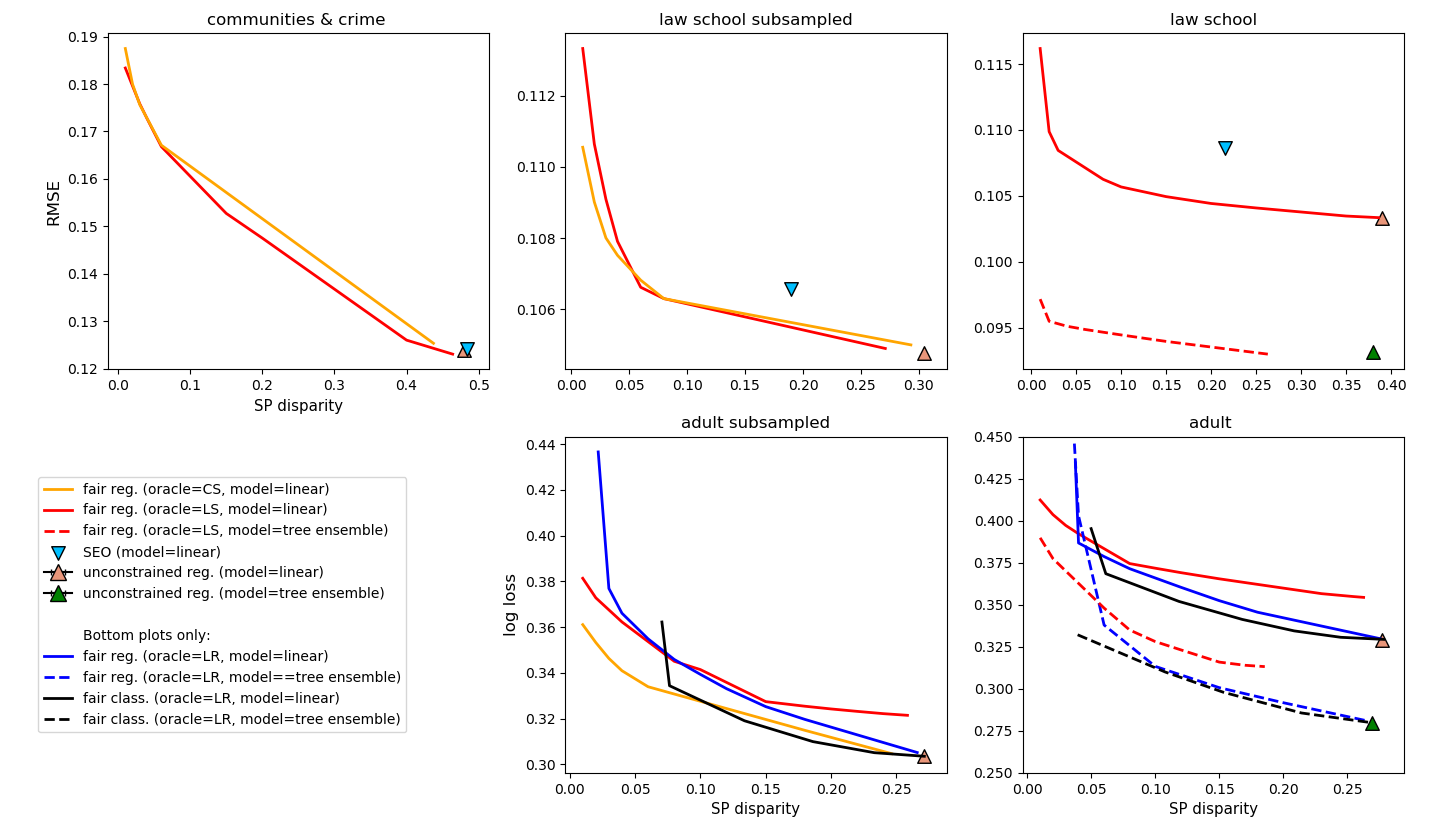
\includegraphics[width=\textwidth, height=9cm]{Figure_2}
\vspace{-8mm}
\caption{Training loss versus constraint violation with respect to
  DP. For our algorithm, we varied the fairness slackness parameter
  and plot the Pareto frontiers of the sets of returned predictors. For the logistic regression experiments, we also plot the Pareto frontiers of the sets of returned predictors given by fair classification reduction methods. }
\label{train}
\end{figure*}

\paragraph{Implementation of the cost-sensitive oracle.}
Given an instance of cost-sensitive classification problem, CS oracle
optimizes the equivalent weighted binary classification problem on the
data $\{W_i, X_i', Y_i\}_{i=1}^n$ with each $X_i' = (x_i, z_i)$ (see
Section \ref{sec:oracles} for the transformation). The oracle aims to
solve
\begin{equation}\label{hard}
\min_{h\in \calH}  \sum_{i=1}^n W_i \mathbf{1}\left\{ h(X_i') \neq Y_i \right\}.
\end{equation}
where every function $h$ in the class $\calH$ is parameterized by a
vector $\beta$ and defined as
$h(x, z) = \mathbf{1}\left\{\langle \beta, x\rangle \geq z\right\}$
for any input $(x, z)$. Instead of optimizing over the objective in
\eqref{hard}, we will consider the following minimization problem with
hinge loss. It will be convenient to consider the labels $Y_i$ take
values $\{\pm 1\}$ and each predictor $h$ predicts in $\{\pm
1\}$. Then the optimization becomes:
\[
  \min_{\beta} \sum_{i=1}^n W_i \max\left\{0, \tfrac{\alpha}{2} -
    \langle \beta, x_i\rangle Y_i\right\}
\]
Furthermore, we will optimize over $\beta$ with $\ell_\infty$ norm
bounded by 1. Then we can encode the optimization problem as a linear
program:
%
\begin{align*}
&\min_{\beta, t} \quad\sum_{i} t_i\\
\mbox{for all }i\in[n]:& \quad t_i \geq 0,\\
\mbox{for all }i\in[n]:& \quad t_i \geq \tfrac{\alpha}{2} - Y_i \, \langle \beta , x_i \rangle,\\
\mbox{for all }j\in[d]:& -1 \leq \beta_j \leq 1.
\end{align*}
%
In our experiments, this optimization problem was solved with the Gurobi Optimizer~\cite{gurobi}.


\paragraph{Runtime comparison.}
We performed a comparison on the running time of a single call of the
three supervised learning oracles. On a subsampled law school data set
with 1,000 examples, we ran the oracles to solve an instance of the
$\BestH$ problem, optimizing over either the linear models or tree
ensemble models. The details are listed in Table~\ref{table}. We also
compare the number of oracle calls for different specified values of
fairness slackness.


\begin{table}
\centering
\begin{tabular}{|l|l|l|}
\hline
Oracle & \begin{tabular}[c]{@{}l@{}}Model\\ class\end{tabular} & \begin{tabular}[c]{@{}l@{}}Runtime per call\\ (seconds)\end{tabular} \\ \hline
CS     & linear                                                & 18.94                                                                \\ \hline
LS     & linear                                                & 3.48                                                                 \\ \hline
LS     & tree ensemble                                         & 3.60                                                                 \\ \hline
LR     & linear                                                & 3.62                                                                 \\ \hline
LR     & tree ensemble                                         & 3.69                                                                 \\ \hline
\end{tabular}
\caption{Runtime comparison on the oracles over different model
  classes. We ran the oracles on a sub-sampled law school data set
  with 1,000 examples, using a machine with a 2.7 GHz Intel processor
  and 16GB memory.}
\label{table}
\end{table}



\begin{figure*}[!t]
  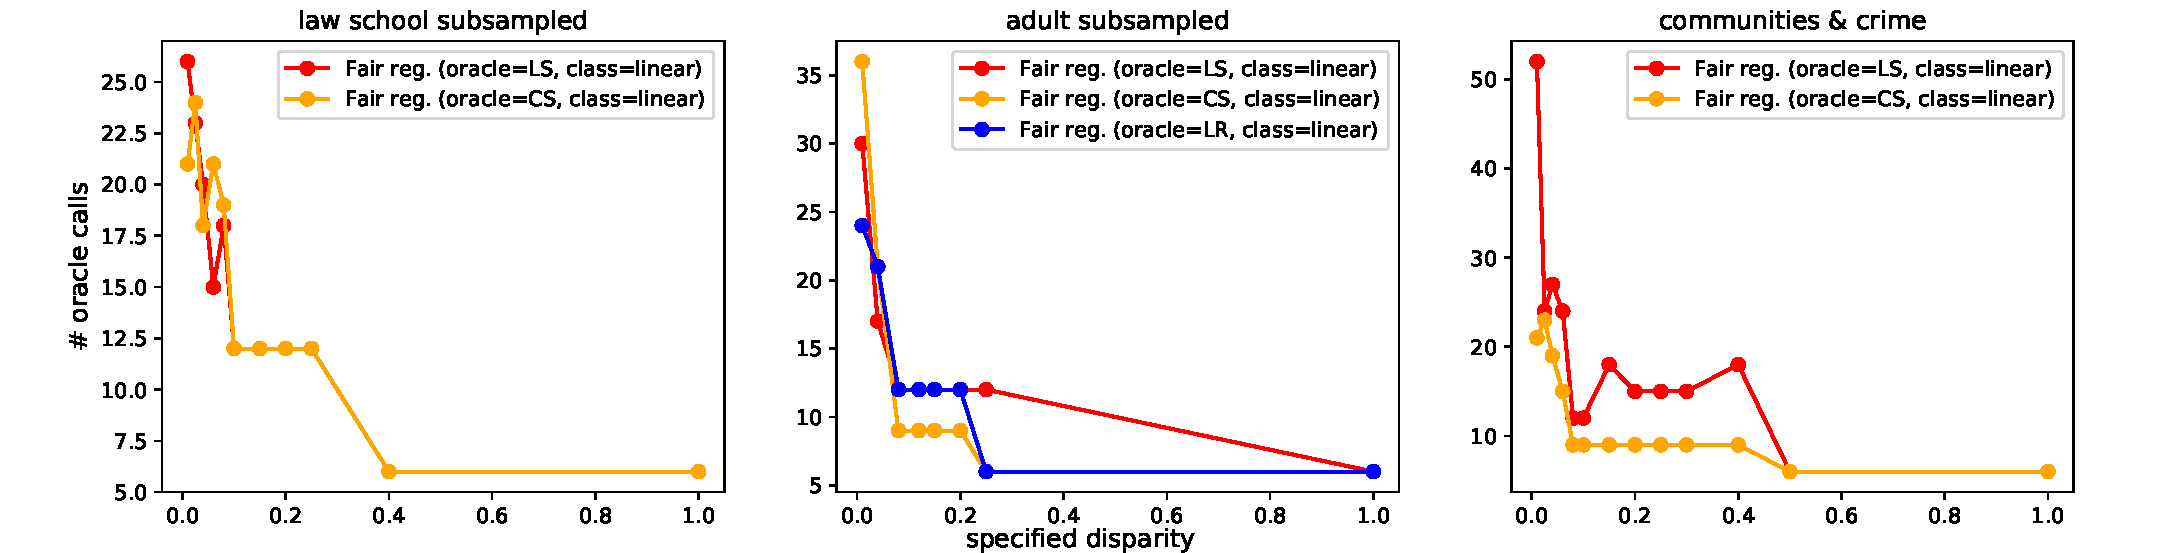
\includegraphics[width=\textwidth, height=4cm]{Ncalls}
\vspace{-8mm}
\caption{Number of oracle calls versus specified value of fairness slackness.}
\end{figure*}




%%% Local Variables:
%%% mode: latex
%%% TeX-master: "main"
%%% End:
